\documentclass[10pt,a4paper]{article}
\usepackage[utf8]{inputenc}
\usepackage{amsmath}
\usepackage{amsfonts}
\usepackage{amssymb}
\usepackage{fullpage}
\usepackage{booktabs}
\usepackage{caption}
\usepackage{subcaption}
\usepackage{graphicx}
\usepackage{epstopdf} 

\author{Christoph Aymanns}
\begin{document}
\section{Definitions}
Let:
\begin{itemize}
\item Adjacency matrix of network: $\mathbf{A}$
\item Neighbourhood of a given node: $B$ 
\item Size of neighbourhood: $k =|B|$: 
\item Number of node in network: $n$.
\item Action vector: $\mathbf{x}$.
\item Private belief: $p$ 
\item Social belief: $q = \sum_{i \in B} x_i / k = \mathbf{A} \mathbf{x} / k$. 
\item Threshold function: $f(p,q)$ such that:
\begin{equation}
x = \begin{cases} 1 &\mbox{if } f(p,q) > 0.5  \\
0 & \mbox{if } f(p,q) < 0.5 \end{cases}
\end{equation}
\end{itemize}
We distinguish between three cases for the threshold function:
\begin{enumerate}
\item ``Equal'':
\begin{equation}
f(p,q) = 0.5(p+q).
\end{equation}
\item ``Neighbor'':
\begin{equation}
f(p,q) = \frac{1}{k+1}p + \frac{k}{k+1}q.
\end{equation}
\item ``Rel Neighbor'':
\begin{equation}
f(p,q) = \left(1 - \frac{k}{n-1}\right) p + \frac{k}{n-1}q.
\end{equation}
\end{enumerate}

\section{Distribution of the private belief}
Based on the signal structure, the Bayesian update of the private belief and the choice of the action we can derive the probability that the agent chooses the state matching action. We begin by deriving the distribution of private beliefs. Suppose the state of the world is $\theta  = 0$. Furthermore note that: 
\begin{itemize}
\item Signal structure:
\begin{equation}
\begin{aligned}
f_0(s) &= \frac{1}{\sqrt{2\pi}\sigma_0} \exp \left( \frac{-(s-\mu_0)^2}{2 \sigma_0^2} \right)\\
f_1(s) &= \frac{1}{\sqrt{2\pi}\sigma_1} \exp \left( \frac{-(s-\mu_1)^2}{2 \sigma_1^2} \right) 
\end{aligned}
\end{equation}
In the following we take $\sigma_0 = \sigma_1 = \sigma$.
\item PDF of signal given $\theta = 0$:
\begin{equation}
p_S(s) = \frac{1}{\sqrt{2\pi}\sigma} \exp \left( \frac{-(s-\mu_0)^2}{2 \sigma^2} \right)
\end{equation}
\item Private belief:
\begin{equation}
p(s) = \left( 1 + \frac{f_0(s)}{f_1(s)} \right)^{-1}
\end{equation}
\item We are interested in the probability distribution of the private belief $p_P(p)$. Let $s(p) = p^{-1}(p)$ be the inverse of the private belief:
\begin{equation}
s(p)=  \frac{\mu_i^2-\mu_1^2+2 \sigma^2 \log \left(\frac{1-p}{p}\right)}{2 (\mu_0-\mu_1)}
\end{equation}
The distribution of the private belief can be computed as follows:
\begin{equation}
p_P(p) = \frac{\partial s(p) }{\partial p } p_S(s(p)).
\end{equation}
Substituting in the expression for $s(p)$ and computing the partial derivative we obtain:
\begin{equation}
p_P(p) = \frac{\left(\left(-\frac{1-p}{p^2}-\frac{1}{p}\right) p \sigma^2\right) \exp \left(-\frac{\left((\mu_0-\mu_1)^2-2 \sigma^2 \log \left(\frac{1}{p}-1\right)\right)^2}{8 \sigma^2 (\mu_0-\mu_1)^2}\right)}{\left(\sqrt{2 \pi } \sigma\right) ((1-p) (\mu_0-\mu_1))}
\end{equation}
\item Now that we have defined the pdf of the private belief we can compute the probability that agent chooses $x=0$ given some social belief $q$ (we use the notation $p_P(p \mid \theta = 0)$ to indicate that the functional form of $p_P$ has be derived assuming that $\theta = 0$:
\begin{equation}
\Pr(x = 0 \mid q = q) = \int_0^{1-q} p_P(p \mid \theta = 0) dp.
\end{equation}
\item Note that in fact this result generalizes to all $\theta$ due to the symmetry of the signal structure. In fact it can be shown (so far only by direct computation):
\begin{equation}
\Pr(x = \theta \mid q = q) = \int_0^{1-q} p_P(p \mid \theta = 0) dp  =\int_{1-q}^1 p_P(p \mid \theta = 1) dp.
\end{equation}
Therefore we have derived an expression for the probability of choosing the correct action that does not depend on the actual state of the world but only on the signal structure and the social belief. Thus we can assume in the following without loss of generality that $\theta = 0$.
\end{itemize}


\begin{figure}[ht]
\centering
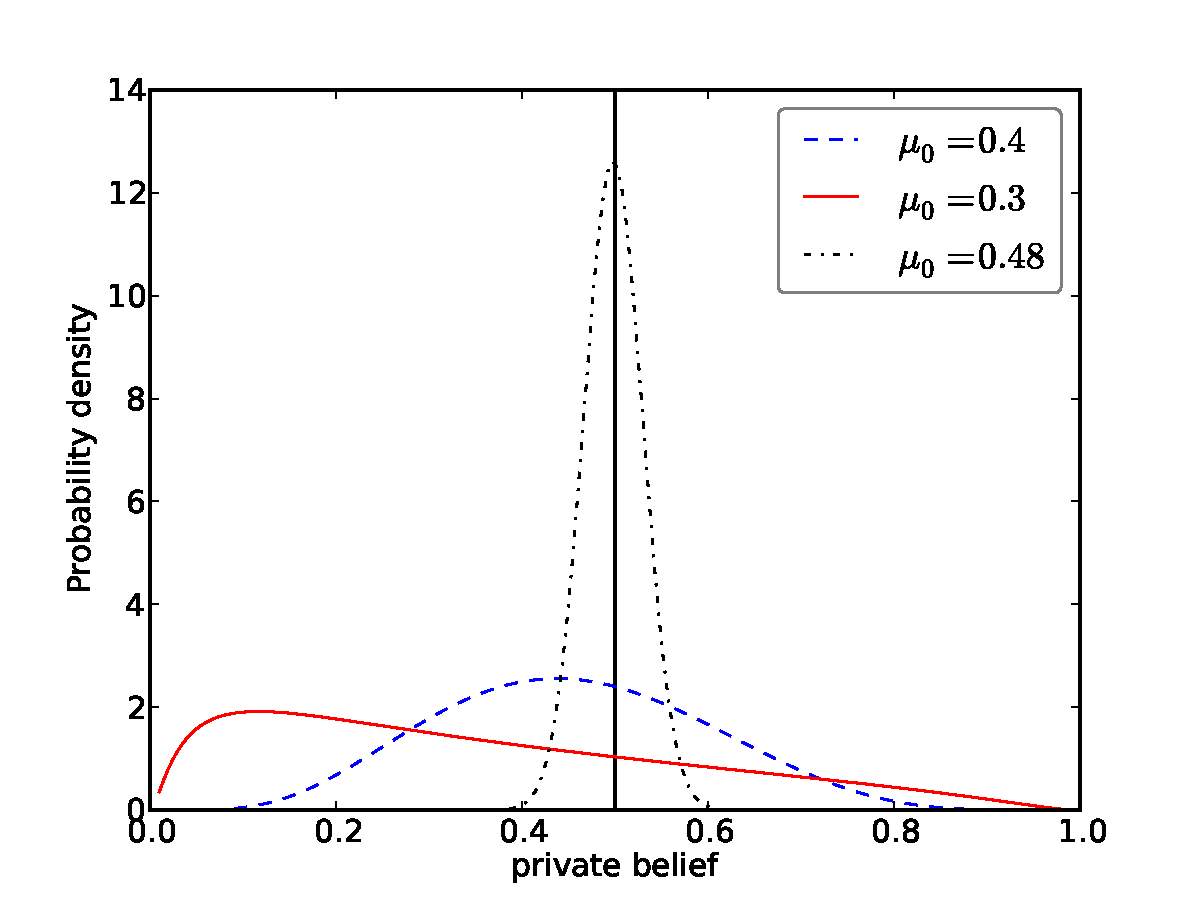
\includegraphics[width=0.5\textwidth]{figures/PRIVATE_BELIEF_DIST}
\caption{Probability density function of the private belief given that the state of the world is $\theta=0$ $p_P(p \mid \theta = 0)$ for three values of $\mu_0 \in \left\lbrace 0.3,0.4,0.48 \right\rbrace$. Furthermore we have $\mu_1 = 1 - \mu_0$ and $\sigma^2 = 0.1$ Note that the majority of the probability density of the private belief is to the left of $0.5$ in all cases. Therefore the private signal tends to produce private beliefs that yield the state matching action. If we increase the $\mid\mu_0 - 0.5\mid$ the distribution becomes more skewed towards zero. Hence the private belief becomes more informative.}
\end{figure}

\section{Mean field considerations}
Given the probability of choosing the state matching action we can attempt to understand the action dynamics in the mean field. We assume that $N \rightarrow \infty$ and that the network is ``fully mixed''. Consider the action of a representative agent. Recall that:
\begin{equation}
x = \begin{cases} 1 &\mbox{if } p+q > 1  \\
0 & \mbox{if } p+q < 1 \end{cases}
\end{equation}
Further recall that the social belief is $q = \sum_{i \in B} x_i / k = \mathbf{A} \mathbf{x} / k$. In the mean field the social belief will simply be the average action of the population:
\begin{equation}
q = \Pr(x = 0 \mid q = q)\times 0 + \Pr(x = 1 \mid q = q)\times 1 = \Pr(x = 1 \mid q = q)
\end{equation}
This yields a self consistency relation for the social belief (and hence for average action of the population). The equilibrium average action $q^*$ is therefore given by the solution of the self consistency relation:
\begin{equation}
q^* = \Pr(x = 1 \mid q = q^*) = \int_{1-q*}^1 p_P(p \mid \theta = 0) dp.
\end{equation}
Note that  $\Pr(x = 1 \mid q = 0) = 0$ and $\Pr(x = 1 \mid q = 1) = 1$. Since $\Pr(x = 1 \mid q = q^*)$ is the cumulative distribution function of the bell shaped private belief it will have a sigmoid shape. Therefore the self consistency equation will have three solutions: $q_1=0$, $q_2=1$ and some $q_3 \in (0,1)$. We illustrate this in figure \ref{FIG::EQ_SOCIAL_BELIEF}. $q_1$, $q_2$ are stable fixed points while $q_3$ is unstable (obvious from figure \ref{FIG::EQ_SOCIAL_BELIEF} and from specified dynamics). $q_3$ defines the ``critical'' social belief beyond which the system synchronizes on the state non-matching action. Note that these dynamics are isomorphic to the Ising model at zero temperature and the Hopfield network model.

\begin{figure}[ht]
\centering
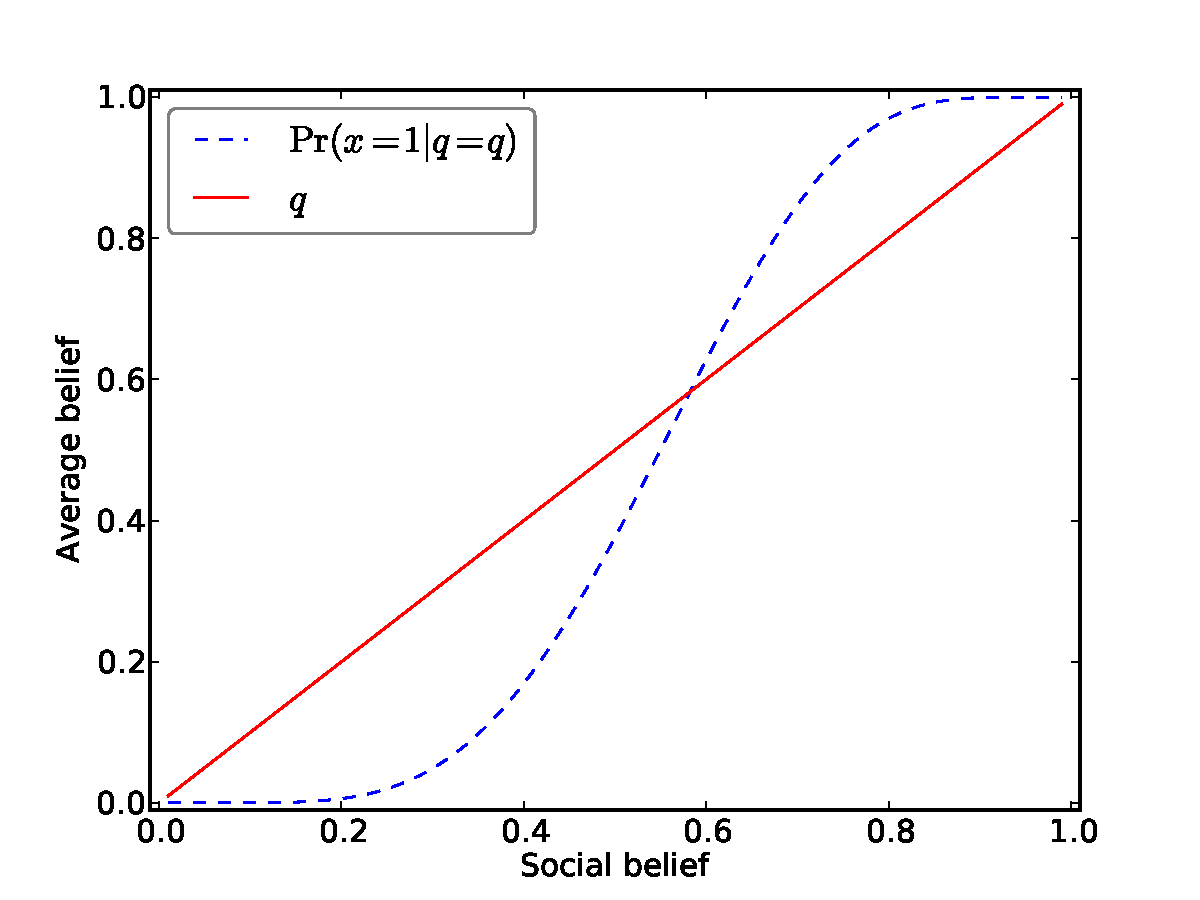
\includegraphics[width=0.5\textwidth]{figures/EQ_SOCIAL_BELIEF}
\caption{Probability of choosing state matching action (equivalent to average social belief and average action in mean field) given that the state of the world is $\theta=0$ $p_P(p \mid \theta = 0)$ for $\mu_0 = 0.4$. Furthermore we have $\mu_1 = 1 - \mu_0$ and $\sigma^2 = 0.1$. The intersections between the probability function and the diagonal mark the fixed points of the system. }
\label{FIG::EQ_SOCIAL_BELIEF}
\end{figure}

\section{Endogenous network formation}
\subsection{Derivation of expected utility}
It is reasonable to assume that the agent has knowledge of the pdf of the private belief - at least he has access to all the relevant information to compute it. In the following I will describe a mechanism for endogenous network formation based on boundedly rational utility maximization.

First consider the expected utility of an agent given some social belief (we assume the agent has some ``belief'' about the social belief, i.e. the average action of his neighbors). Recall that the utility is:
\begin{equation}
u(x) = \begin{cases} 1 &\mbox{if } x= \theta  \\
0 & \mbox{if } x \neq \theta\end{cases}
\end{equation}
The expected utility conditional on some $q$ is hence:
\begin{equation}
\bar{u}(q) = \Pr(x = \theta \mid q = q),
\end{equation}
recall that above we derived an expression for this that only depends on the signal structure and not the actual state of the world. The agent cannot change his private belief. However, he can try to change his social belief by choosing his neighbors. In order to evaluate the marginal utility from adding a new neighbor the agent must reason about how the probability of choosing the correct action changes when adding a new neighbor. Of course the change will be in $q$.

This set up clearly suggests an equilibrium concept in which the neighbor's beliefs again depend on their social belief leading to an infinite regress. Rather than going down that route we assume that the agent has some simple constant belief about the social belief of his neighbors $q'$. If completely ignorant about his neighbors' neighbors he would assume that $q'=0.5$. Alternatively he could assume that $q'=q$. For the rest of this document we will assume that $q'=0.5$.

The expected utility of agent $i$ conditional on some $q'$ and neighborhood $B_i$ is (note that we basically shifted the conditionality to our neighbor's neighborhood):
\begin{equation}
\bar{u}_i(q',B_i) = \sum_{a \in Q_i} \Pr(q_i = a \mid q') \Pr(x_i = \theta \mid q_i = a),
\end{equation}
where $Q_i$ is the set of all possible values for the social belief of agent $i$. For a given size of the agent's neighborhood $k_i$ this set is simply given by $Q_i = \{n/k_i \mid n \in \mathbb{Z}, n \geq 0, n \leq k_i \}$. The probability of a particular social belief can be computed by summing over the probabilities of combinations of actions chosen by the neighbors of agent $i$. Define the set of feasible action vectors of $i$'s neighbors conditional on some social belief $a$: $X_{ai} = \{\mathbf{x} \mid \sum_j x_j = a, x_j \in \{0,1\}, j\in B_i\}$.
\begin{equation}
\label{EQ::1}
\Pr(q_i = a \mid q') = \sum_{\mathbf{y} \in  X_{ai}} \prod_{j \in B_i} \Pr(x_j = y_j \mid q_j = q').
\end{equation}
Define the probability that neighbor $j$ chooses the state matching action:
\begin{equation}
z_j = \Pr(x_j = \theta \mid q_j = q') = \int_0^{1-q_j} p_{P_j}(p_j \mid \theta = 0) dp
\end{equation}
Note that $p_{P_j}(p_j \mid \theta = 0)$ will depend on the signal structure of neighbor $k$. Now we can write for the probability in equation \ref{EQ::1}:
\begin{equation}
\Pr(x_j = y_j \mid q_j = q') = \begin{cases} z_j &\mbox{if } y_j = 0  \\
1-z_j & \mbox{if } y_j = 1 \end{cases}
\end{equation}
Note that if $z_j = z \forall j$ the distribution in \ref{EQ::1} would be a simple binomial distribution. However in general this is not the case.

\subsection{Network formation process}
Now we have all the ingredients to compute the expected utility of an agent given his neighborhood and $q'$. In the endogenous network formation proposed here the agent will seek to maximize this probability by changing his neighborhood while holding $q'$ fixed. Before explaining the algorithm for endogenous network formation note that:
\begin{itemize}
\item If there is no cost to maintaining a link, the utility maximizing network will be fully connected.
\item However, in the presence of a cost for maintaining a link, there will be some network density that depends on the cost per link. Note that marginal utility of an additional link decreases with the number of links. This is because the expected utility is bounded by 1 (pay-off is 1 and probability of choosing the correct action is less than or equal to 1). I think that in the limit of $N \rightarrow \infty$ one should be able to show that the resulting network density is always $\rho < 1$ for some cost $c > 0$. Maybe this is trivial though. When the marginal utility of adding a new link is less than the cost of maintaining the link the agent will not add the new link.
\end{itemize}
In the following we assume that the cost of maintaining a link is constant (i.e. not a function of the number of links).

The network formation algorithm is as follows:
\begin{itemize}
\item Choose a random agent $i$ from the set of agents $\mathcal{A}$.
\item Choose another agent $j$ randomly from the set of agents that are not yet neighbors of $i$ $\mathcal{A} \setminus B_i $. We choose an agent $j$ with the following probability:
\begin{equation}
w_j = \exp(\beta E_j)/Z,
\end{equation}
where $Z = \sum_k w_k$. $E_j = |0.5-\mu_{0j}|$ is a proxy for agent $j$'s signal strength. For $\beta = 0$ $i$ chooses the new agent with equal probability. This probability can be justified if we assume that the agent has some noisy knowledge of the signal strength of the other agents before contacting them.
\item Let $B_i' =  B_i \cup j$, i.e. the neigborhood of agent $i$ after adding adding agent $j$. Similarly $B_j' =  B_j \cup i$.
\item The marginal utilities of adding $j$ and $i$ to the respective neighborhoods are then:
\begin{equation}
\begin{aligned}
\Delta \bar{u}_i(q',B_i',B_i) &= \bar{u}_i(q',B_i')-\bar{u}_i(q',B_i) \\
\Delta \bar{u}_j(q',B_j',B_j) &= \bar{u}_j(q',B_j')-\bar{u}_j(q',B_i) 
\end{aligned}
\end{equation} 
\item The network formation process is subject to the pairwise stability condition, i.e. a link will only be formed if it is beneficial to both agents. Given the marginal utilities of agents $i$ and $j$ and their cost of maintaining link $c_i$ and $c_j$  we have:
\begin{enumerate}
\item If $\Delta \bar{u}_i(q',B_i',B_i) > c_i$ and $\Delta \bar{u}_j(q',B_j',B_j) > c_j$: Form link.
\item If $\Delta \bar{u}_i(q',B_i',B_i) > c_i$ and $\Delta \bar{u}_j(q',B_j',B_j) < c_j$:
\begin{itemize}
\item Find least informative agent in neighborhood of $j$: $l = \underset{m \in B_j}{\operatorname{argmin}}$ $E_m $.
\item Define $B_j'' = B_j' \setminus l$.
\item If $\Delta \bar{u}_i(q',B_i',B_i) > c_i$ and $\Delta \bar{u}_j(q',B_j'',B_j) > c_j$: Form link $ij$ and remove link $jl$.
\item Otherwise: Don't form link.
\end{itemize}
\item If $\Delta \bar{u}_i(q',B_i',B_i) < c_i$ and $\Delta \bar{u}_j(q',B_j',B_j) > c_j$: Do as above but with $i\rightarrow j$ and $j\rightarrow i$.
\item If $\Delta \bar{u}_i(q',B_i',B_i) < c_i$ and $\Delta \bar{u}_j(q',B_j',B_j) < c_j$: Combine the two above.
\end{enumerate}
\end{itemize}

\section{Results}
The network formation algorithm described above can lead to quite a large variety of networks. In the case of homogeneous agents not much interesting will happen and the result of the network formation algorithm will be an ER network. The density of the network will be a function of the agent's signal strength and the cost of maintaining a link. For low costs the network will be close to fully connected.

However there are also some parameter configurations in which interesting network structures are possible. Here we will consider the following configuration: There are a few ``informed'' agents with strong signals and low costs of maintaining a link. The majority of the population will be ``uniformed'' with relatively weak signals and higher costs of maintaining a link.
\begin{table}[h]
\begin{tabular}{llr} 
\toprule
Notation & Description & Value \\
\midrule
$N$ & Number of agents & $30$\\
$N_I$ & Number of informed agents & $4$\\
$N_U$ & Number of unformed agents & $26$\\
$\mu_{0I}$ & Average signal for $\theta = 0$ for informed agents& $0.3$\\
$\mu_{1I}$ & Average signal for $\theta = 1$ for informed agents& $0.7$\\
$\sigma_{0I}$ & Standard deviation of signal for $\theta = 0$ for informed agents& $\sqrt{0.1}$ \\
$\sigma_{1I}$ & Standard deviation of signal for $\theta = 1$ for informed agents& $\sqrt{0.1}$ \\
$\mu_{0U}$ & Average signal for $\theta = 0$ for uninformed agents& $0.4$\\
$\mu_{1U}$ & Average signal for $\theta = 1$ for uninformed agents& $0.7$\\
$\sigma_{0U}$ & Standard deviation of signal for $\theta = 0$ for uninformed agents& $\sqrt{0.1}$ \\
$\sigma_{1U}$ & Standard deviation of signal for $\theta = 1$ for uninformed agents& $\sqrt{0.1}$ \\
$c_{I}$ & Cost per link for informed agent& $0$\\
$c_{U}$ & Cost per link for informed agent& $0.1$\\
$T_C$ & Number of iterations of network algorithm & $400$ \\
$q'$ & Agent's belief of average action of neighbors of neighbors & $0.5$ \\
$\beta$ & Intensity of choice in agent selection & $30$ \\
\midrule
$T$ & Number of iterations of action updater & $100$ \\ 
$n$ & Number of endogenously formed networks used for simulation & $1000$ \\ 
$S$ & Number of simulations per parameter configuration & $100$ \\
$\rho$ & Average density of ER networks & $0.08$ \\ 
\bottomrule 
\end{tabular}
\caption{Parameters for network formation and runs with endogenous and ER networks.}
\end{table}

\begin{figure}[ht]
\centering
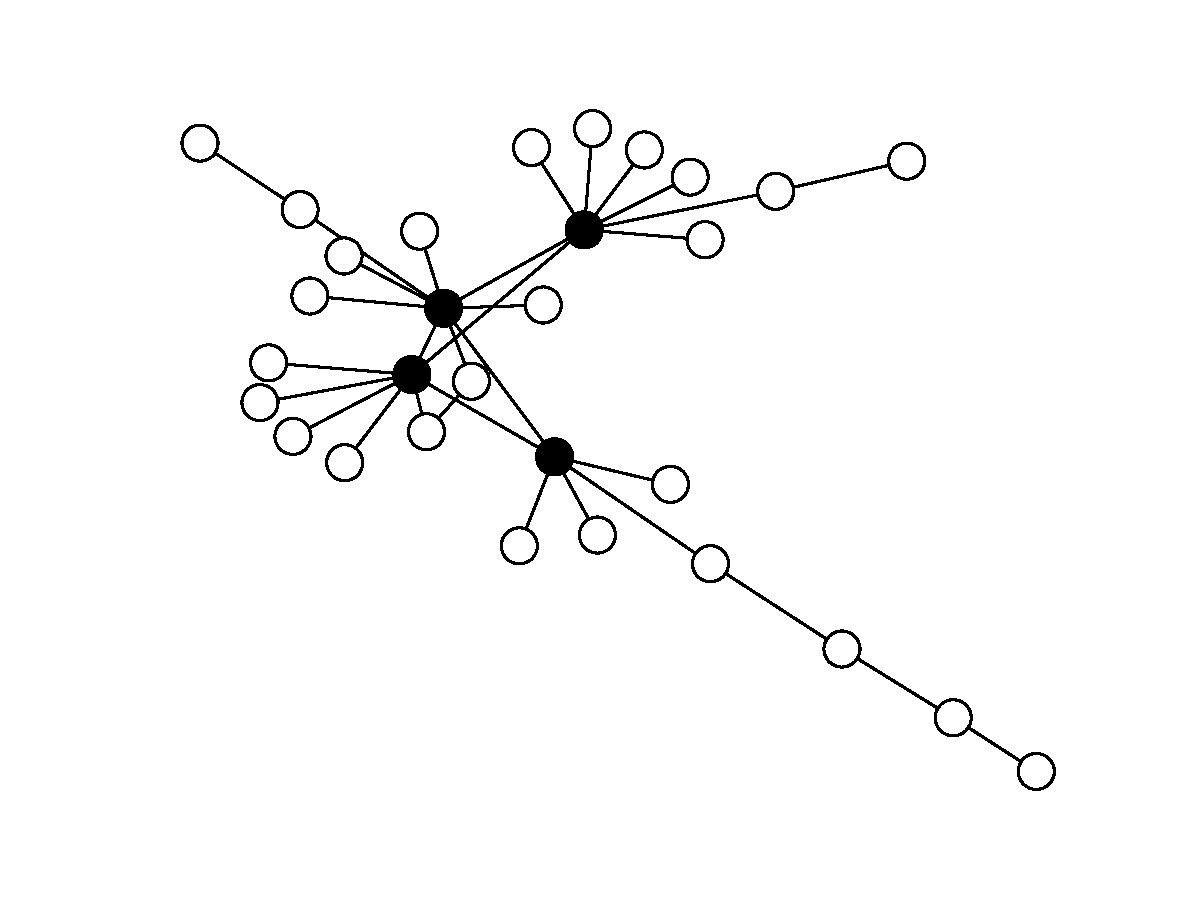
\includegraphics[width=0.7\textwidth]{figures/EXAMPLE_GRAPH_1}
\caption{Example network from ensemble of $n$ endogenously formed networks. Black nodes are ``informed'' agents, while white nodes are ``uninformed''.}
\label{FIG::EXAMPLE_GRAPH_1}
\end{figure}

\clearpage
In order to compare the dynamics on the endogenous networks to the ER networks we run the following simulations:
\begin{itemize}
\item First we created 1000 networks using the network formation algorithm.
\item Then we run the social learning algorithm holding the networks constant. 
\item We also run the social learning algorithm with an initialization bias in which we set the initial action of all agents to some value.
\item We compare the performance of the endogenously formed networks to the performance of ER networks.
\end{itemize}
Note that I have not yet run learning and network formation together. All runs are done using the ``Equal'' threshold function.

\begin{figure}[ht]
\centering
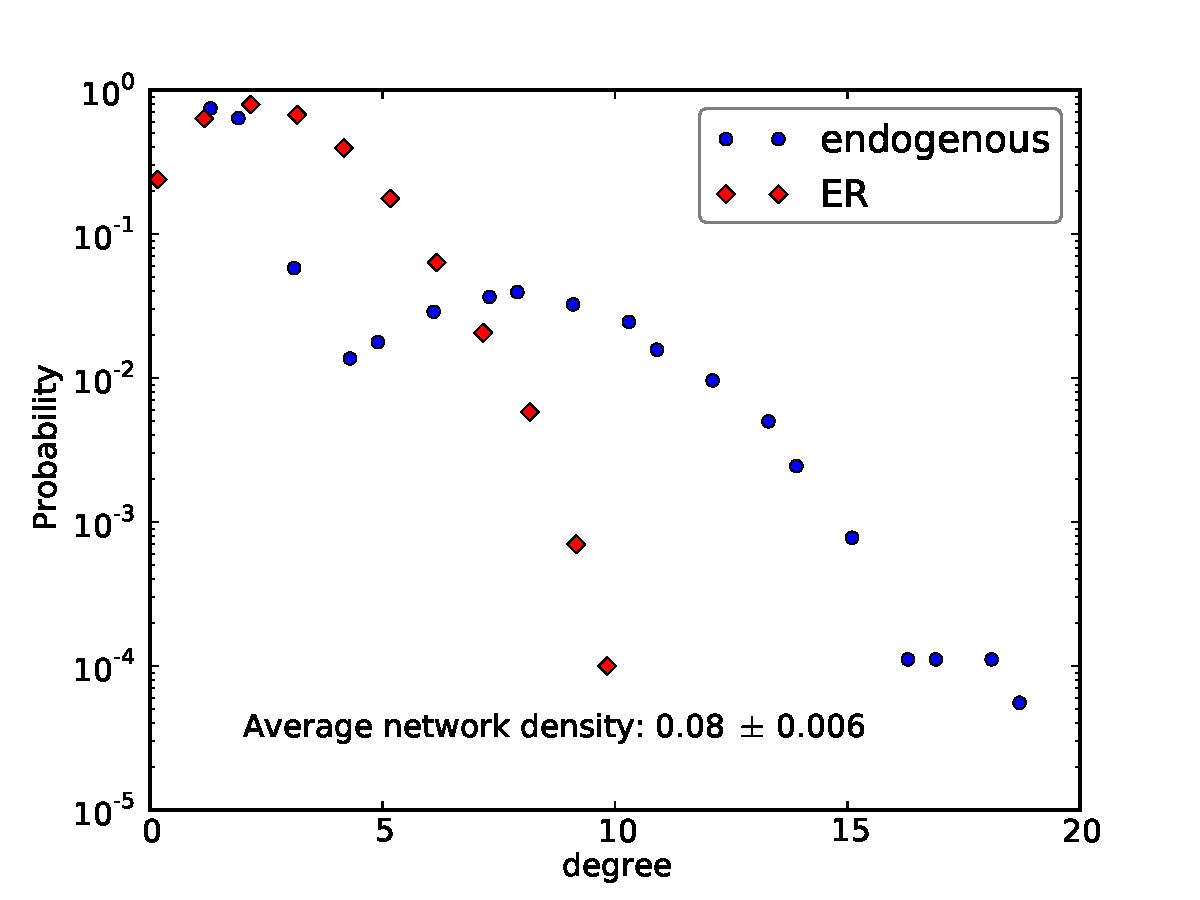
\includegraphics[width=0.5\textwidth]{figures/ENDO_DEGREE_DIST}
\caption{Degree distribution of ensemble of $n$ endogenously formed networks compared to ER networks with same average density. The degree distribution of the endogenously formed networks is clearly bimodal. One peak corresponds to the uninformed nodes with small degree while the second peak corresponds to the informed nodes with high degree.}
\label{FIG::ENDO_DEGREE_DIST}
\end{figure}

\begin{figure}[ht]
\centering
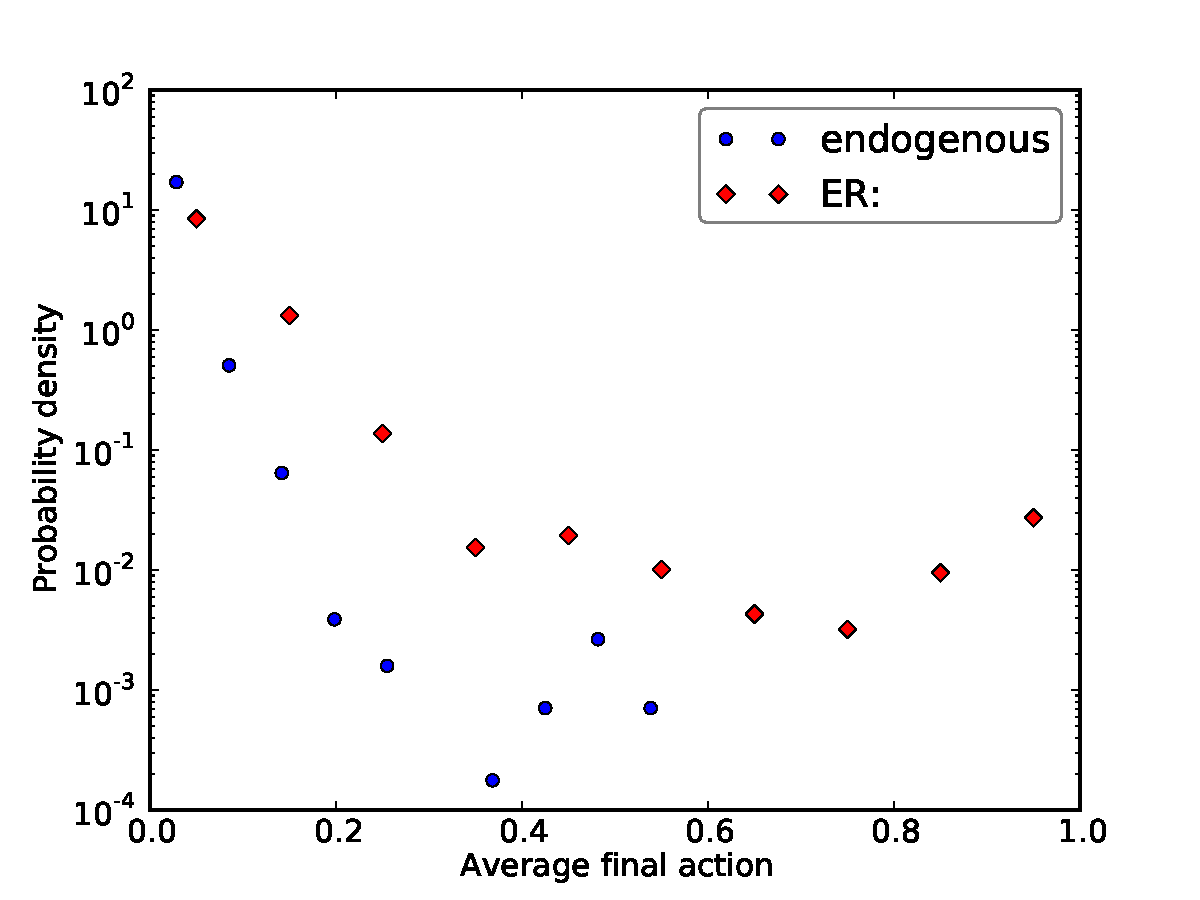
\includegraphics[width=0.5\textwidth]{figures/ENDO_X_FINAL_DIST}
\caption{Distribution of final action ER networks vs. endogenous networks. This is without bias, i.e. the initial action is random based on the private belief only.}
\label{FIG::ENDO_X_FINAL_DIST}
\end{figure}

\begin{figure}[ht]
\centering
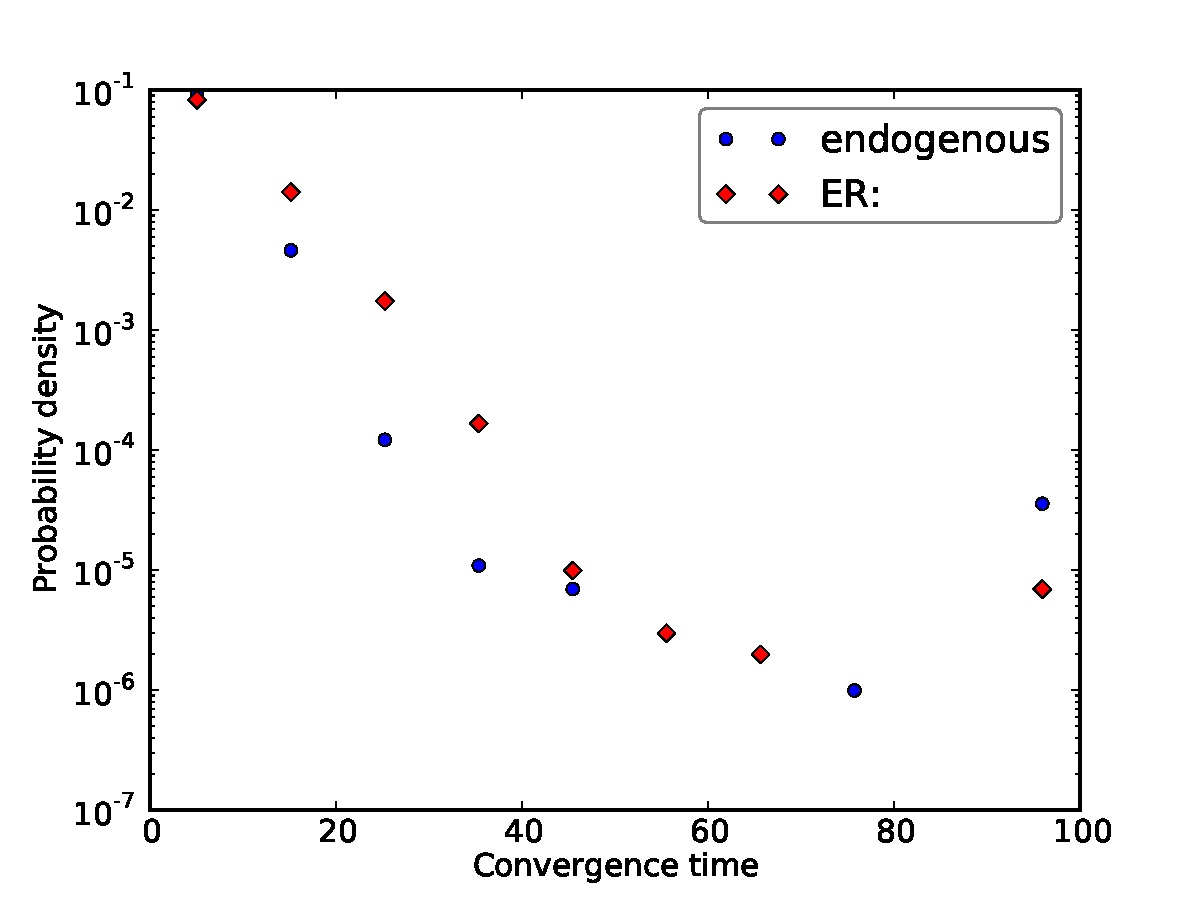
\includegraphics[width=0.5\textwidth]{figures/ENDO_CONV_T_DIST}
\caption{Distribution of convergence time ER networks vs. endogenous networks. This is without bias, i.e. the initial action is random based on the private belief only. We assume the learning has converged at time $t$ if $\sum_i| x_i(t) - x_i(t+dt) | / N < 0.05$, where $dt = 15$.}
\label{FIG::ENDO_CONV_T_DIST}
\end{figure}

\begin{figure}[ht]
\centering
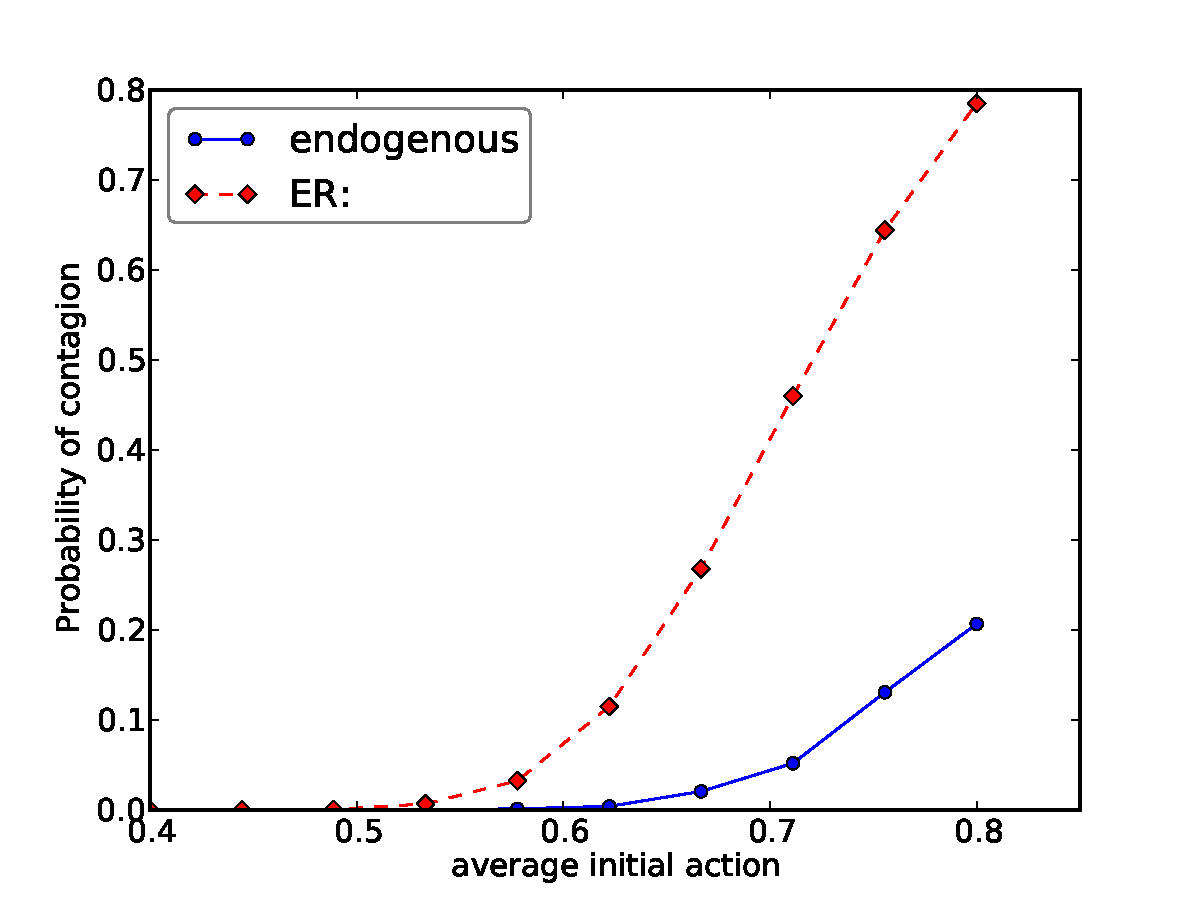
\includegraphics[width=0.5\textwidth]{figures/ENDO_P_CONT}
\caption{Probability of contagion vs. initialization bias.}
\label{FIG::ENDO_P_CONT}
\end{figure}

\begin{figure}[ht]
\centering
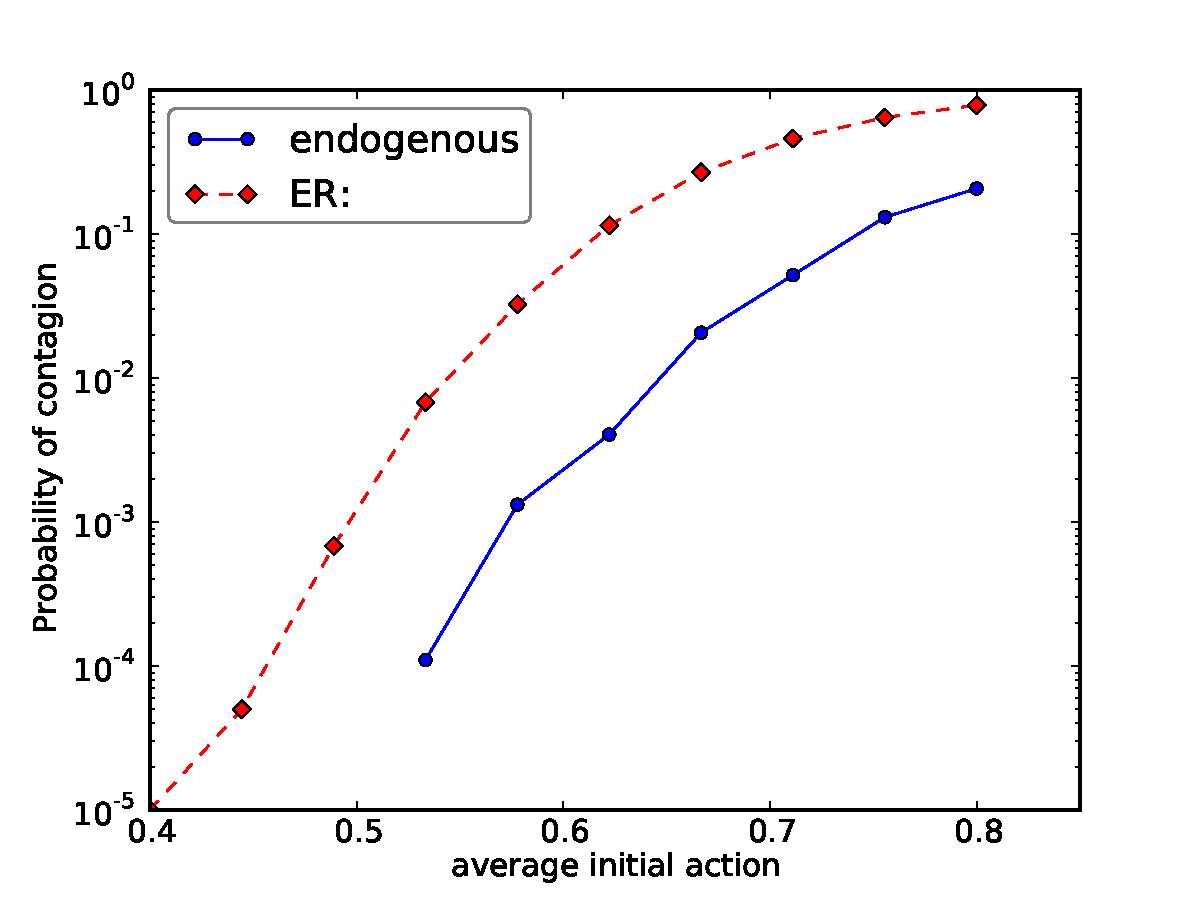
\includegraphics[width=0.5\textwidth]{figures/ENDO_P_CONT_LOG}
\caption{Probability of contagion vs. initialization bias. This is the same as above just on a log scale. Missing values correspond to zero frequency.}
\label{FIG::ENDO_P_CONT_LOG}
\end{figure}

\end{document}